\chapter{Methods}
\label{cha:Methods}


% Doku für APseudocode package
% https://ftp.agdsn.de/pub/mirrors/latex/dante/macros/latex/contrib/pseudocode/pseudocode.pdf

\renewcommand{\thepseudonum}{\roman{pseudonum}}
\begin{pseudocode}{Collect Data}{ }
\COMMENT{Fill RolloutBuffer with samples obtained by current model}\\

\PROCEDURE{CollectData}{}
num\_steps \GETS 0\\
RolloutBuffer.\CALL{Reset}{}\\
Env.\CALL{Reset}{}\\
\WHILE RolloutBuffer\CALL{NotFull}{} \DO
\BEGIN
obs \GETS Env.\CALL{GetObservation}{}\\
action \GETS Model.\CALL{GetAction}{obs}\\
reward \GETS Env.\CALL{Step}{action}\\
num\_steps \GETS num\_steps + 1\\
\CALL{AddToRolloutBuffer}{obs, action, reward}\\
\IF Env.\CALL{IsFinished}{} \THEN
Env.\CALL{Reset}{}\\
\END\\
\RETURN{num\_steps}
\ENDPROCEDURE

\end{pseudocode}

\begin{figure}
     \centering
     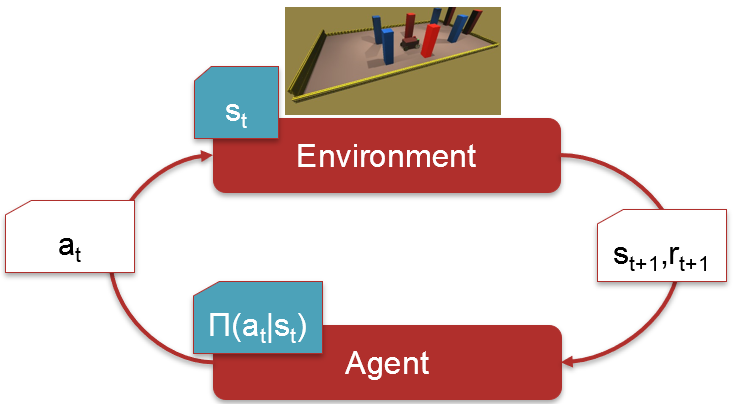
\includegraphics[width=0.8\textwidth]{Bilder/rl_cycle.png}
     \caption{Loop in Collect Data}
     \label{fig:unitycommunication}
\end{figure}


\renewcommand{\thepseudonum}{\roman{pseudonum}}
\begin{pseudocode}{Train Model}{ }
\COMMENT{Sample from replay buffer and update the model based on the loss}\\

\PROCEDURE{TrainModel}{}
amount\_of\_batches \GETS \frac{rollout\_buffer\_size}{batch\_size}\\
\FOR i \GETS 0 \TO n\_epochs \DO
\BEGIN
RolloutBuffer.\CALL{Shuffle}{}\\
\FOR i \GETS m \TO amount\_of\_batches \DO
\BEGIN
batch \GETS RolloutBuffer.\CALL{GetBatch}{m}\\
loss \GETS \CALL{ComputeLoss}{batch}\\
Model.\CALL{Backpropagate}{loss}\\
Optimizer.\CALL{Step}{}\\
\END\\
\END
\ENDPROCEDURE

\end{pseudocode}



\renewcommand{\thepseudonum}{\roman{pseudonum}}
\begin{pseudocode}{Evaluate Model}{ }
\COMMENT{Evaluate Model on tracks of all difficulties}\\

\PROCEDURE{Episode}{}
\WHILE Env.\CALL{IsFinished}{}==False \DO
\BEGIN
obs \GETS Env.\CALL{GetObservation}{}\\
action \GETS Model.\CALL{GetAction}{obs}\\
\END\\
\IF Env.\CALL{FinishedSuccessfully}{} \THEN
success \GETS 1
\ELSE
success \GETS 0\\
\RETURN{success}
\ENDPROCEDURE

\PROCEDURE{EvalModelTrack}{n\_episodes, difficulty}
successful\_episodes \GETS 0\\
\FOR episodes \GETS 0 \TO n\_episodes \DO
\BEGIN
Env.\CALL{Reset}{difficulty}\\
successful\_episodes \GETS successful\_episodes + \CALL{Episode}{}\\
\END\\
success\_rate \GETS \frac{successful\_episodes}{n\_eval\_episodes}\\
\RETURN{success\_rate}
\ENDPROCEDURE

\PROCEDURE{EvalModel}{}
easy\_success\_rate = \CALL{EvalModelTrack}{n\_episodes=num\_evals\_per\_difficulty, \\difficulty=''easy''}\\
medium\_success\_rate = \CALL{EvalModelTrack}{n\_episodes=num\_evals\_per\_difficulty, \\difficulty=''medium''}\\
hard\_success\_rate = \CALL{EvalModelTrack}{n\_episodes=num\_evals\_per\_difficulty, \\difficulty=''hard''}\\
\\
total\_success\_rate = (easy\_success\_rate + medium\_success\_rate + hard\_success\_rate) / 3\\
\IF total\_success\_rate > best\_success\_rate \THEN
\BEGIN
best\_success\_rate \GETS total\_success\_rate\\
Model.\CALL{SaveToFile}{}\\
\END
\ENDPROCEDURE
\end{pseudocode}

\renewcommand{\thepseudonum}{\roman{pseudonum}}
\begin{pseudocode}{TrainNetwork}{ }
\label{Train}
\COMMENT{Main Training Algorithm}\\

\MAIN
Env \GETS \CALL{Environment}{environment\_parameters}\\
RolloutBuffer \GETS \CALL{RolloutBuffer}{rollout\_buffer\_size}\\
Model \GETS \CALL{Model}{model\_parameters}\\
Optimizer \GETS \CALL{Optimizer}{optimizer\_parameters}\\


num\_timesteps \GETS 0\\
iteration \GETS 0\\
\WHILE num\_timesteps < total\_timesteps \DO 
\BEGIN 
num\_steps \GETS \CALL{CollectData}{}\\
num\_timesteps \GETS num\_timesteps + num\_steps\\
iteration \GETS iteration + 1\\
\CALL{TrainModel}{}\\
\IF iteration \mathbin{\%}  log\_interval = 0 \THEN
\BEGIN
success\_rate \GETS \CALL{EvalModel}{}\\
\CALL{LogToTensorboard}{key=''eval/success\_rate'', value=success\_rate,\\ step=num\_timesteps}\\
\END
\END\\
\ENDMAIN
\end{pseudocode}


